% This document is licensed, at your option, under these or any newer versions of these licenses:
% Creative Commons Attribution 3.0 Unported License
% Creative Commons Attribution 4.0 International License
%
% You should have received a copy of the license along with this work. If not, see:
% <http://creativecommons.org/licenses/by/3.0/>
% <http://creativecommons.org/licenses/by/4.0/>

\documentclass{isprs}
\usepackage{subfigure}
\usepackage{setspace}
\usepackage{geometry} % added 27-02-2014 Markus Englich
\usepackage{epstopdf}
\usepackage{url}
\usepackage[dvipsnames]{xcolor}
\usepackage[colorlinks, allcolors=Blue]{hyperref}
%\usepackage[pdfborderstyle={/S/U/W 1}, citebordercolor=purple, urlbordercolor=blue]{hyperref}
%\usepackage{natbib}

\geometry{a4paper, top=25mm, left=20mm, right=20mm, bottom=25mm, headsep=10mm, footskip=12mm} % added 27-02-2014 Markus Englich
%\usepackage{enumitem}

%\usepackage{isprs}
%\usepackage[perpage,para,symbol*]{footmisc}

%\renewcommand*{\thefootnote}{\fnsymbol{footnote}}



\begin{document}

\title{VALIDATION STRATEGY COMPARISON FOR PLS REGRESSIONS}

\author{
 D. Masili\=unas\textsuperscript{a}}

\address
{
	\textsuperscript{a }Wageningen University, Droevendaalsesteeg 3, NL 6708 PB, Wageningen, The Netherlands - dainius.masiliunas@wur.nl
}

\icwg{}   %This field is NOT optional after all.

\abstract
{
To be added.
}

\keywords{To, Be, Determined}

\maketitle

\section{INTRODUCTION}\label{INTRODUCTION}

Validation is an important step in the model creation process, as it determines how well the model performs in practice and whether it is reliable enough for the required use-case. Validation also gives insight into how many samples of the population need to be taken to achieve a certain model accuracy level.

There are two types of model validation: holdout (true, conventional) validation and cross-validation. In holdout validation, the total sample set is divided into two subsets: a training (model building) and validation (test) sets. Only the training set is used for creating the model. The validation set is put aside, in order to more realistically assess the model performance after it is created. The drawback to holdout validation is that by holding back some of the samples, the sample size from which a model is derived becomes smaller, and thus the model accuracy suffers. In order to achieve the same level of accuracy as when not doing holdout validation, extra samples equal to the validation set size need to be collected, which can be a costly and time-consuming task.

In contrast, in cross-validation, all available samples in the model are used. The validation step is made possible by temporarily splitting the full sample set into training and validation sets, as in holdout validation, but it is repeated a number of times with different ways of splitting, so that every sample goes in both the training and validation set at least once. Then a summary statistic is calculated and used to determine the model accuracy. The drawback to cross-validation is that since all samples are used in the model, it cannot be utilised as a way to optimise the model for better external validity by dropping samples without worthwhile information from the training set. In addition, cross-validation tends to produce overly optimistic results, since the model takes the samples used for validation into account.

There are numerous strategies for splitting the samples into training and validation sets for each of the validation types. There have been studies comparing them \cite{clark2003boosted}, but to date there has not been a comprehensive study comparing validation methods when applied specifically to the hyperspectral models used in earth observation. In this paper, the effectiveness of a number of different cross-validation and holdout validation strategies on Partial Least Squares Regression (PLSR) models have been assessed. In particular, we take a look at how cross-validation techniques influence the selection of the number of components to use when building the model, and how model accuracy scales with sample size when different holdout validation techniques are applied.

\section{METHODS}\label{sec:METHODS}

\subsection{Cross-validation strategies}\label{sec:Cross-validation strategies}

In order to assess how cross-validation techniques influence the selection of the number of components, the R package \textit{plsr} was used, specifically the function \textit{validationplot()} with different cross-validation parameters available in the package. Tested cross-validation sampling stategies were: Leave-one-out (LOO), random, Monte Carlo random, interleaved and consecutive. For sampling strategies other than LOO, the full data set was divided into two subsets validated against each other. If the number of subsets increases, the result gets closer and closer to LOO cross-validation result (see figure \ref{fig:interleaved-group-sizes}).

\begin{figure}[ht!]
\begin{center}
    %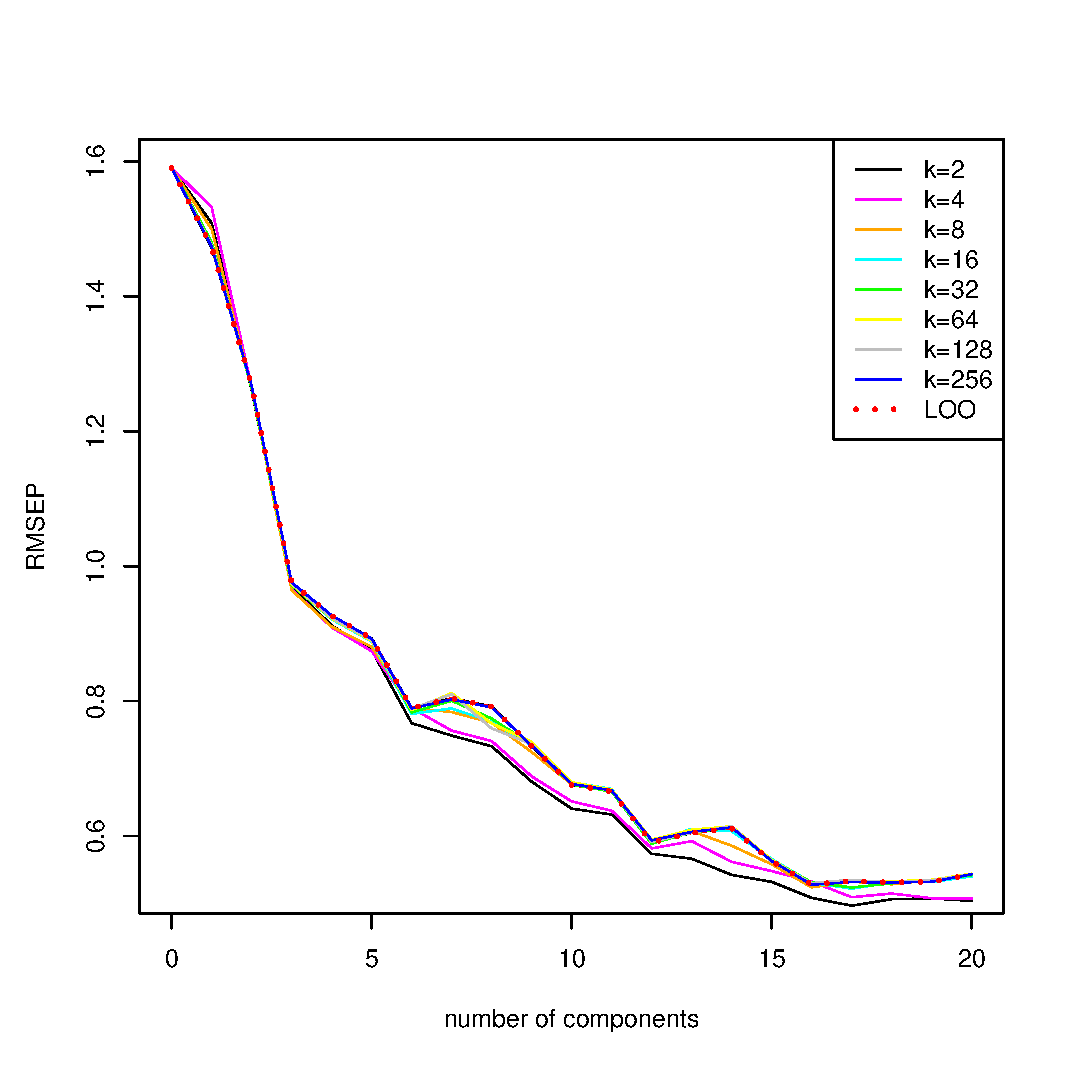
\includegraphics[width=1.0\columnwidth]{../script/output/interleaved-group-sizes.eps}
    \caption{Interleaved cross-validation result with different number of cross-validation subsets \textit{k}.}
    \label{fig:interleaved-group-sizes}
\end{center}
\end{figure}

\subsection{Holdout validation strategies}\label{sec:Holdout validation strategies}

For assessing holdout validation techniques, samples were split into training and validation sets manually for random, interleaved and stratified sampling. For the respective Monte Carlo sampling, the splitting into different sets was repeated 100 times, and the result was averaged over all runs. For Kennard-Stone sampling, the R package \textit{inspectr} was used to generate the validation sample set, based on the Kennard-Stone algorithm \cite{kennard1969computer}. For OptiSim sampling \cite{clark1997optisim}, the latest in-development code from the \textit{inspectr} package was used. OptiSim sampling was run using k = 4, since studies have shown that it generally performs the best on hyperspectral datasets \cite{clark2003boosted}.

\subsection{Data}\label{sec:Data}

The model used for this paper was created by using the Netherlands soil spectra dataset, using the \textit{plsr} package. For assessing the external performance of the resulting models, the Australian soil spectra dataset \cite{rossel2010using}, provided in the \textit{inspectr} package, was used as a validation set.

\section{RESULTS}\label{sec:RESULTS}


\section{DISCUSSION}\label{sec:DISCUSSION}

{%\footnotesize
	\begin{spacing}{0.9}% tune the size by altering the parameter
		\bibliography{AEO-paper}
	\end{spacing}
}

\section*{APPENDIX}\label{APPENDIX}

The R code used to carry out the analysis for this paper is available online, at:

\url{https://github.com/GreatEmerald/AEO-validation-paper}

\end{document}
